\section{Модификация проекта «Выпуклая оболочка»}
\subsection*{4.1 Постановка задачи}
В следующем проекте решалась задача вычисления расстояния от заданной прямой
до выпуклой оболочки. Кроме того, необходимо определять выпуклую оболочку и
 вычислять её характеристики сразу после поступления очередной точки. Для наглядного
  отображения работы программы необходимо графически иллюстрировать каждый этап,
   используя графический интерфейс Tk.

\subsection*{4.1 Теоретические аспекты}

 Пусть $X$~--- множество $\mathbb{R}^2$ точек плоскости,
  а $P$~--- совокупность всех выпуклых фигур на плоскости.
   Тогда тройка функций $f\colon X^* \rightarrow \mathcal{P}$ — выпуклая оболочка
    последовательности точек, $g\colon X^* \rightarrow \mathbb{R}$  — её периметр
     и  $h\colon X^* \rightarrow \mathbb{R}$ — её площадь, задаёт индуктивную
функцию $F\colon X^* \rightarrow \mathcal{P} \times \mathbb{R} \times \mathbb{R},$ $F = \begin{pmatrix}f\\ g\\ h\end{pmatrix}.$

 Пусть для некоторой последовательности точек плоскости выпуклая оболочка,
  а также её периметр и площадь, уже известны. Тогда после добавления
новой точки $x\in X$ возможны две ситуации: либо точка $x$ попадает внутрь оболочки,
 либо вне её.

Для получения новой оболочки необходимо, как это хорошо видно
 из следующего рисунка, удалить все освещённые рёбра, а концы оставшейся ломаной
  соединить двумя новыми рёбрами с добавляемой точкой $x$:
\begin{figure}[ht!]
\begin{center}
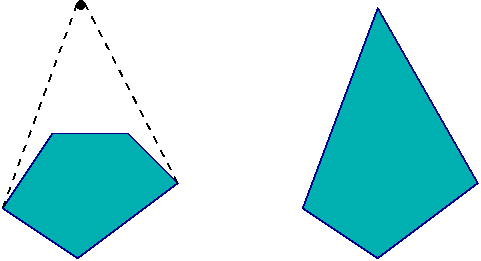
\includegraphics[width=0.4\hsize]{images/conv_2}
\end{center}
\caption{Удаление освещённых рёбер}\label{fig:conv_2}
\end{figure}

Если добавляемая точка лежит на продолжении одного из рёбер,
 то оболочка должна измениться, поэтому ребро, на продолжении которого лежит
  точка мы также будем считать освещённым:

\begin{figure}[ht!]
\begin{center}
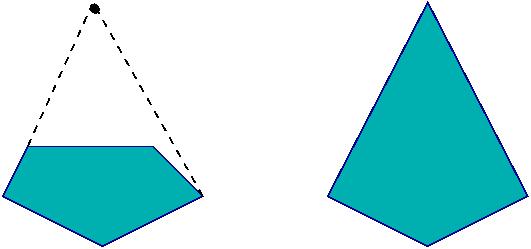
\includegraphics[width=0.4\hsize]{images/conv_3}
\end{center}
\caption{Удаление освещённых рёбер}\label{fig:conv_3}
\end{figure}

Для работы с точками на плоскости создаётся класс \verb|R2Point|. В нём необходим ряд
методов, которые позволяли бы вычислять \verb|расстояния| между точками,
сравнивать их на \verb|совпадение|, выяснять, лежат ли три точки на одной
прямой, находится ли некоторая точка на прямой \verb|между| двумя другими,
пересекаются ли отрезки, а также вычислять расстояние от заданной
прямой до выпуклой оболочки, сравнивая \verb|расстояние до отдельных рёбер|.
Кроме того, необходимо уметь вычислять \verb|площадь треугольника| и находить
все \verb|освещённые| ребра многоугольника.

Для вычисления площади треугольника в данном случае разумнее всего будет
воспользоваться векторным произведением $S = \frac{1}{2} |\vec a \times \vec b|$.
Тогда сократится количество необходимых вычислительных операций и результат будет более точным,
по сравнению с аналогичными способами вычисления.

Для векторов  $\vec a = (a_x, a_y, a_z)$ и $\vec b = (b_x, b_y, b_z)$  координаты вектора
 $\vec c$ находятся по формуле \\
\begin{center}
$\vec c = \left| \begin{array}{ccc} \vec i& \vec j& \vec k\\ a_x & a_y & a_z \\ b_x & b_y & b_z \end{array} \right| =$ $= (a_y b_z - a_z b_y) \vec i + (a_z b_x - a_x b_z) \vec j + (a_x b_y - a_y b_x) \vec k$.
\end{center}
Однако в том случае, когда векторы $\vec a$ и $\vec b$ расположены на плоскости,
их векторное произведение имеет единственную отличную от нуля компоненту,
вычисление которой и должно быть реализовано в методе \verb|area|.
Также важно то, что вычисляемая площадь является \verb|ориентированной|,
то есть может быть отрицательной.

Для вычисления расстояния от точки до прямой используется метод \verb|dist_to_line|.
 В его основу положена хорошо известная формула:

 $$d = \frac{|A\times M_x+B\times M_y+C|}{\sqrt{A^2+B^2}}$$. Коэффициенты  \verb|A|, \verb|B| и \verb|C|
 мы получаем из общего вида уравнения прямой, проходящей через две точки:
   $ \left(y_1-y_2\right)x+\left(x_2-x_1\right)y+\left(x_1y_2-x_2y_1\right)=0. $

Ниже приведена реализация метода \verb|dist_to_line|:

\begin{lstlisting}
 def dist_to_line(m,n)
    a = (n.y-m.y)
    b = (m.x-n.x)
    c = m.x*(m.y-n.y)+m.y*(n.x-m.x)
    ((a*@x+b*@y+c).abs/Math.sqrt(a*a+b*b))
 end
\end{lstlisting}


\subsection*{4.1 Описание используемых структур и применяемых алгоритмов}

Определение того факта, лежат ли три точки на одной прямой (это делает
метод \verb|triangle?|), сводится к вычислению площади треугольника
и сравнению её с нулём; а для того, чтобы точка $T$ прямой находилась на отрезке
$[A,B]$ этой же прямой (проверяет справедливость этого факта
метод экземпляра \verb|inside?|), необходимо и достаточно принадлежности
проекций этой точки проекциям на оси координат отрезка $[A,B]$.

Для того чтобы реализовать метод \verb|light?|, позволяющий выяснить,
освещено ли ребро $[A,B]$ выпуклой оболочки из данной точки, дадим строгое определение освещённости.
Ребро [A,B] называется освещённым из точки $T$, если ориентированная
площадь треугольника, образованного точками $A, B$ и $T$ отрицательна, либо если
точка $T$ расположена на прямой, проходящей через точки $A$ и $B$ вне отрезка [A,B].

Искомое расстояние от заданной прямой до выпуклой оболочки будет отлично от нуля
в том случае, если прямая не пересекает ни одно ребро данного многоугольника.
Метод \verb|intersect?| будет вычислять взаимное расположение
отрезков, заданных точками класса \verb|R2Point|, при помощи векторных произведений.

Пусть даны два отрезка. Первый задан точками $P_1(x_1;y_1)$ и $P_2(x_2;y_2)$.
 Второй задан точками $P_3(x_3;y_3)$ и  $P_4(x_4;y_4)$.

\begin{figure}[ht!]
\begin{center}
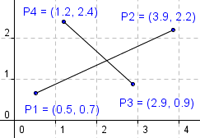
\includegraphics[width=0.4\hsize]{images/conv_4}
\end{center}
\caption{Взаимное расположение отрезков}\label{fig:conv_4}
\end{figure}

\newpage
Тогда их взаимное расположение проверяется с помощью векторных произведений
 (каждое из них реализуется методом \verb|cross|):
\begin{center}
$v_1 = |\vec {P_3P_4} \times \vec {P_3P_1}|, $
$v_2 = |\vec {P_3P_4} \times \vec {P_3P_2}|$

$v_3 = |\vec {P_1P_2} \times \vec {P_1P_3}|, $
$v_4 = |\vec {P_1P_2} \times \vec {P_1P_4}|$.
\end{center}
Рассмотрим отрезок $P_3P_4$ и точки $P_1$ и $P_2$.

\begin{figure}[ht!]
\begin{center}
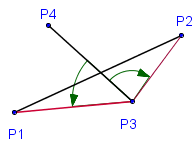
\includegraphics[width=0.5\hsize]{images/conv_5}
\end{center}
\caption{}\label{fig:conv_5}
\end{figure}

Точка $P_1$ лежит слева от прямой $P_3P_4$. Для неё
векторное произведение

 $v_1 = |\vec {P_3P_4} \times \vec {P_3P_1}| > 0,$
так как векторы положительно ориентированы.
Точка $P_2$ расположена справа от прямой $P_3P_4$. Для неё
 векторное произведение

 $v_2 = |\vec {P_3P_4} \times \vec {P_3P_2}| < 0,$
 так как векторы отрицательно ориентированы.

Для того чтобы точки $P_1$ и $P_2$ лежали по разные стороны от прямой $P_3P_4$,
 достаточно, чтобы выполнялось условие $v_1v_2 < 0$ (векторные произведения имели противоположные  знаки).

Аналогичные рассуждения можно провести для отрезка $P_1P_2$ и точек $P_3$ и $P_4$.

Итак, если $v_2 = |\vec {P_3P_4} \times \vec {P_3P_2}| < 0,$ то отрезки пересекаются.

Ниже представлена реализация указанных методов:

\begin{lstlisting}

 def cross(w)
    @x*w.y-w.x*@y
 end

 def R2Point.intersect?(a,b,c,d)
    h = R2Point.new((d.x-c.x),(d.y-c.y))
    j = R2Point.new((a.x-c.x),(a.y-c.y))
    k = R2Point.new((b.x-c.x),(b.y-c.y))
    return true if h.cross(j)*h.cross(k) < 0
    false
 end
\end{lstlisting}


Далее необходимо определить контейнер для хранения точек выпуклой оболочки.
 Наиболее подходящим в данном случае является дек, так как его можно свернуть
  в кольцо и считать <<текущим>> то ребро оболочки, которое соединяет начало и конец дека.
   Дальнейшие операции проводятся применительно к этому ребру:

\begin{figure}[ht!]
\begin{center}
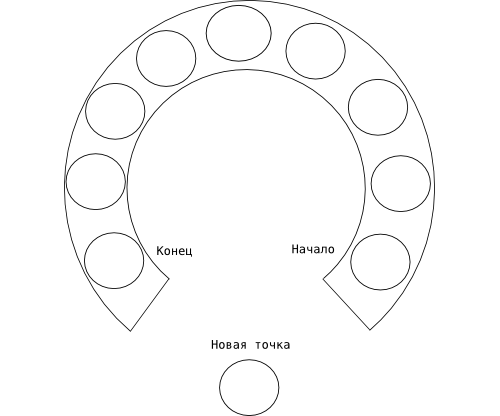
\includegraphics[width=0.6\hsize]{images/conv_6}
\end{center}
\caption{Дек, содержащий точки}\label{fig:conv_6}
\end{figure}
 Для того чтобы удалить все освещенные ребра необходимо, <<повернуть>> дек таким образом,
  чтобы концы одного из освещённых рёбер находились в конце и в начале дека соответственно
  (если только освещённые рёбра вообще существуют). После этого нужно удалить найденное ребро.


Проектирование основных классов выполнено следующим образом:
 cоздаётся базовый класс \verb|Figure| (фигура), и из него выводятся необходимые
  нам классы: \verb|Void| (нульугольник), \verb|Point| (одноугольник),
   \verb|Segment| (двуугольник) и \verb|Polygon| (многоугольник).

\begin{figure}[ht!]
\begin{center}
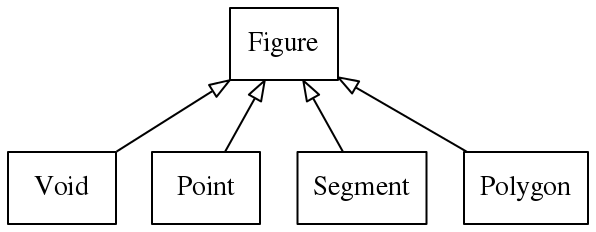
\includegraphics[width=0.7\hsize]{images/conv_7}
\end{center}
\caption{Иерархия классов}\label{fig:conv_7}
\end{figure}

Каждый из последних четырёх классов должен реализовывать методы \verb|add| (добавить новую точку),
\verb|perimeter| (получить периметр выпуклой оболочки) и \verb|area| (получить площадь выпуклой оболочки).
 При этом объект типа \verb|Point| должен содержать внутри себя одну точку (компоненту
  типа \verb|R2Point|), объект типа \verb|Segment|~--- две, а типа \verb|Polygon|~--- целый дек точек.

Вернемся к цели данной модификации, а именно~--- вычислению расстояния
 от заданной прямой до выпуклой оболочки. Прежде всего, мы будем хранить 2 точки,
  задающие прямую, как экземпляры класса \verb|Figure|: @@apoint, @@bpoint.
   Нужный параметр @@d(расстояние) следует переопределять для каждой фигуры,
    начиная с одноугольника. Ниже приведен листинг, демонстрирующий модификацию конкретных
     классов программы.
Для \verb|Segment|:
\begin{lstlisting}
def initialize(p, q)
  @p, @q = p, q
  @@intersect = R2Point.intersect?(@p,@q,@@apoint,@@bpoint)
  @@d = 0.0 if @@intersect
  if @q.dist_to_line(@@apoint,@@bpoint)<@@d && !@@intersect
    @@d = @q.dist_to_line(@@apoint,@@bpoint)
  end
...
end
\end{lstlisting}

Для \verb|Polygon|:
\begin{lstlisting}
...
if c.dist_to_line(@@apoint,@@bpoint)<@@d && !@@intersect
@@d = c.dist_to_line(@@apoint,@@bpoint)
end
...
\end{lstlisting}

При этом, в случае добавления двух новых рёбер в дек искомое расстояние изменится,
 а следовательно, его необходимо перевычислить. В случае пересечения прямой и
 выпуклой оболочки расстояние необходимо приравнять к нулю.
\begin{lstlisting}
...
@intersect=R2Point.intersect?(t,@points.first,@@apoint,@@bpoint)

if !@@intersect
 @@intersect=R2Point.intersect?(t,@points.last,@@apoint,@@bpoint)
end

@@d = 0.0 if @@intersect

if t.dist_to_line(@@apoint,@@bpoint)<@@d && !@@intersect
  @@d = t.dist_to_line(@@aline,@@bline)
end

@points.push_first(t)
...
\end{lstlisting}


\subsection*{4.2 Постановка задачи}
В следующем проекте решалась задача вычисления радиуса максимального круга с
центром в заданной точке, содержащегося в выпуклой оболочке. Кроме того, необходимо
определять выпуклую оболочку и вычислять её характеристики сразу
после поступления очередной точки.
Для наглядного отображения работы программы необходимо
графически иллюстрировать каждый этап, используя графический интерфейс Tk.
\subsection*{4.2 Теоретические аспекты}

Помимо вышеописанных методов и алгоритмов, используемых в выполнении
 предыдущей модификации, необходимо индуктивно
 вычислять максимальный радиус вписанной окружности, т.е. минимальное из  расстояний
  от заданного центра до каждого из рёбер выпуклой оболочки.


\subsection*{4.2 Описание используемых структур и применяемых алгоритмов}\
В общем случае необходимо искать минимальное из расстояний
от заданного центра до каждого ребра выпуклой оболочки (если центр лежит внутри многоугольника).
Если же центр окружности находится вне оболочки~--- радиус вписанной окружности будет равен нулю.



 В первую очередь, необходимо  объявить экземпляр класса \verb|Figure| для центра окружности,
  и метод, который будет вычислять искомый радиус:
\begin{lstlisting}
@@center = nil
def radius; @@R end
\end{lstlisting}

Далее, при первом же вычислении радиуса многоугольника необходимо проверить, лежит ли центр
 внутри выпуклой оболочки:

\begin{lstlisting}
def outside?
   @points.size.times do
     break if @@center.light?(@points.last, @points.first)
     @points.push_last(@points.pop_first)
   end
   @@center.light?(@points.last, @points.first)
end
\end{lstlisting}

Для общего случая будем сразу выполнять эту проверку и в случае надобности   обнулять переменную  @@R, отвечающую за радиус:
\begin{lstlisting}
  outside?() ?  @@R = 0 :  @@R = [@@center.dist_to_line(a,b),
  @@center.dist_to_line(b,c),@@center.dist_to_line(a,c)].min

\end{lstlisting}

Ниже приведён графический вывод работы программы для заданных точек:
\begin{figure}[ht!]
\begin{center}
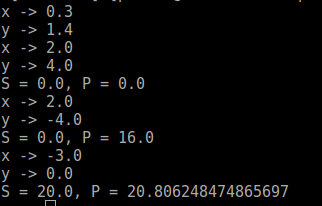
\includegraphics[width=0.5\hsize]{images/poly}
\end{center}
\caption{Ввод данных}\label{fig:poly}
\end{figure}

\begin{figure}[ht!]
\begin{center}
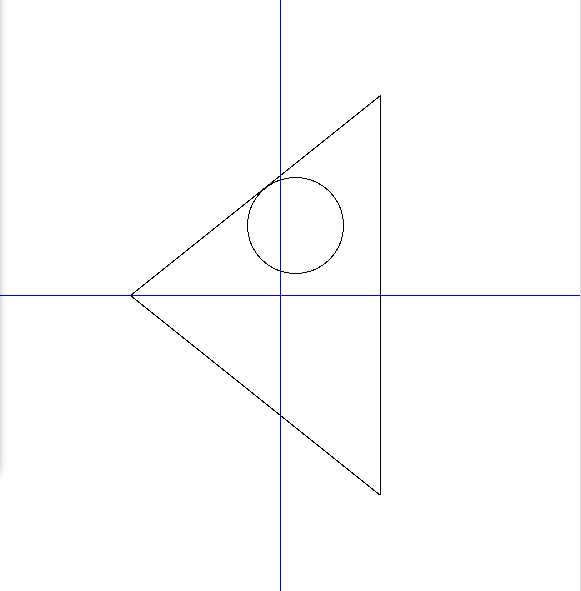
\includegraphics[width=0.5\hsize]{images/poly1}
\end{center}
\caption{Вывод в Tk}\label{fig:poly1}
\end{figure}


 В приложении приведены  реализации некоторых технических моментов, связанных с изменением выпуклой оболочки.


